\documentclass[tikz,border=6pt]{standalone}
\usepackage[T1]{fontenc}
\usepackage{helvet}
\renewcommand{\familydefault}{\sfdefault}
\usetikzlibrary{positioning,arrows.meta,calc}
\begin{document}
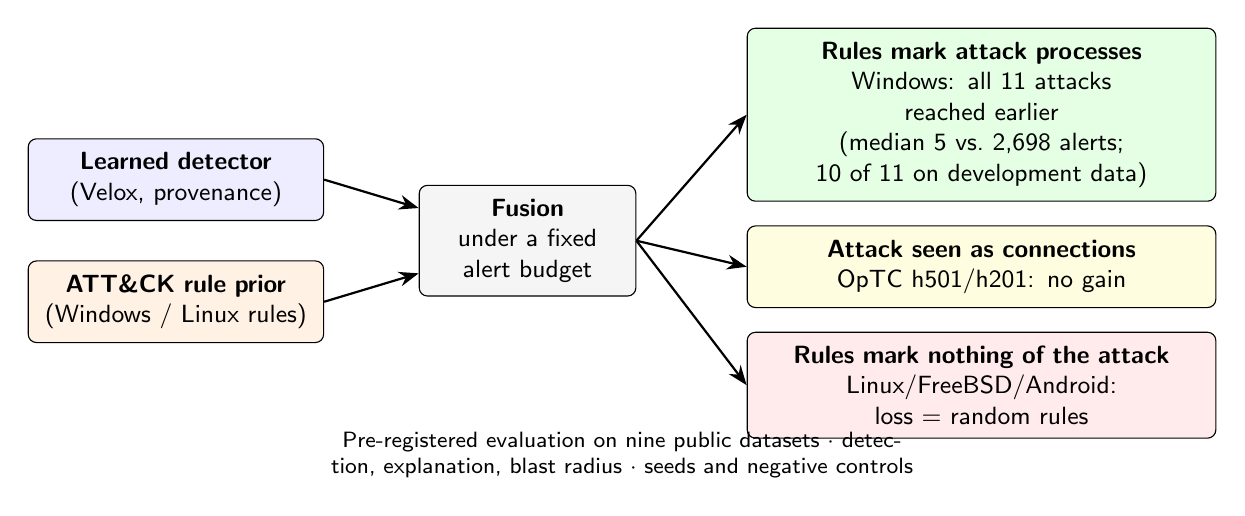
\begin{tikzpicture}[font=\small, node distance=5mm and 8mm,
  box/.style={draw, rounded corners=3pt, align=center, inner sep=5pt, text width=#1}, box/.default=3.4cm,
  arr/.style={-{Stealth[length=2.5mm]}, thick}]
\node[box, fill=blue!7] (l) {\textbf{Learned detector}\\(Velox, provenance)};
\node[box, fill=orange!10, below=of l] (r) {\textbf{ATT\&CK rule prior}\\(Windows / Linux rules)};
\node[box=2.4cm, anchor=west, fill=gray!8] (f) at ($(l.east)!0.5!(r.east)+(12mm,0)$) {\textbf{Fusion}\\under a fixed\\alert budget};
\draw[arr] (l.east) -- (f); \draw[arr] (r.east) -- (f);
\node[box=5.6cm, anchor=west, fill=green!10] (o1) at ($(f.east)+(14mm,16mm)$) {\textbf{Rules mark attack processes}\\Windows: all 11 attacks\\reached earlier\\(median 5 vs.\ 2{,}698 alerts;\\10 of 11 on development data)};
\node[box=5.6cm, below=3mm of o1, fill=yellow!12] (o2) {\textbf{Attack seen as connections}\\OpTC h501/h201: no gain};
\node[box=5.6cm, below=3mm of o2, fill=red!8] (o3) {\textbf{Rules mark nothing of the attack}\\Linux/FreeBSD/Android: loss = random rules};
\draw[arr] (f.east) -- (o1.west); \draw[arr] (f.east) -- (o2.west); \draw[arr] (f.east) -- (o3.west);
\node[anchor=north, align=center, font=\footnotesize, text width=12.5cm] at ($(r.south west)!0.5!(o3.south east)+(0,-4mm)$) {Pre-registered evaluation on nine public datasets $\cdot$ detection, explanation, blast radius $\cdot$ seeds and negative controls};
\end{tikzpicture}
\end{document}
